\documentclass[12pt]{article}
\usepackage[margin=1in]{geometry}
\usepackage{amsmath, amssymb, amsthm, graphicx, hyperref}
\usepackage{enumerate}
\usepackage{fancyhdr}
\usepackage{multirow, multicol}
\usepackage{tikz}
\pagestyle{fancy}
\fancyhead[RO]{Eliot Brown}
\fancyhead[LO]{MA-UY 2314: Discrete Mathematics}
\usepackage{comment}


\begin{document}

I hope you find this file useful.  Throughout the semester, I will upload a tex file in the Homework folder that will help you with LaTex.  

\begin{enumerate}
\item[$\bullet$] Create a project on Overleaf.com.  Delete what you see in the tex file on overleaf and feel free to copy/paste any of my homework tex files into the blank page on Overleaf.  
    \item [$\bullet$]  The region above $\backslash$begin$\{$document$\}$ is called the preamble. This consist of user packages that are required for certain syntax to run.  
    \item[$\bullet$] In the preamble you will see $\backslash$fancyhead$[$RO$]\{$Spring 2020$\}$.  Replace Spring 2020 with your name.  Your name will now appear on each pdf of your pdf.
    \item[$\bullet$] To obtain a pdf, you will compile the tex file.  When ready you will download upload the pdf  onto Gradescope, you must assign a page to each homework problem.  Gradescope has plenty of videos on how to submit homework.  
\end{enumerate}


\section{Homework 0}

Many of you have asked how to hand write question 2 in homework 0. 
\begin{enumerate}
    \item [(1)] Hand write the statement on a blank sheet of paper.  Print your name and sign your name where appropriate.  
    \item [(2)] Take a picture and upload the image onto Overleaf.  The image must be in the same folder as the homework assignment.  The syntax you see below in the tex file is needed to include the jpg file.    
\end{enumerate}

\[
\includegraphics[width = 5in, height = 4in]{yourfile.jpg} %your jpg file goes between the curly brackets.  To size it, play around with the syntax between the square brackets.  
\]

\section{Homework 1}

Here is some sytax associated to homework 1 that will help you.   Your answer does not have to be written exactly like below.  I included the syntax so that you can associated certain syntax with certain Latex symbols.  
\vspace{.15in} %Note that \vspace{.15in} gives us a vertical space of size .15in.  

\noindent 3.1(a) $3|100$ = \textbf{F}.  There is no $k \in \mathbb{Z}$ such that $100 = 3k$.
\vspace{.15in}


\noindent 3.1(b) $3|99$= \textbf{T}.  Notice that $99 = 3k$
where $k = 33$.  
\vspace{.15in}




Below you will find the syntax associated to a truth table.  Just copy/paste the code below into your latex file.  Now adjust the table to the size needed.  If you need another column, use the syntax $|$c$|$c$|$c$|$c$|$ in the code below. 

\[ %centers the table.
\begin{tabular}{|c|c|c|} 
\hline %\hline gives us a horizontal line.  
$x$ & $y$ & $x \rightarrow y$ \\ %the syntax \\ ends the row.
\hline
T & T & T \\
\hline 
T & F & F \\
\hline
F & T & T  \\
\hline
F & F & T \\
\hline
\end{tabular} %end of the table.  
\] %need to close of the center of the table.  



Let's do another problem using Theorem 7.2.  Suppose we have to prove that 
\[ %centers the math text 
(x \vee y) \rightarrow z = (x \rightarrow z) \wedge (y \rightarrow z) %don't need $ signs when math text is between the square brackets.  
\] %need to close the center
using Theorem 7.2.  Let's do it here.  
\[
\begin{aligned} %I want the math text below to align along the & symbol.  I placed my & symbol before the equal sign, but you can place it where ever you wish. 
(x \vee y) \rightarrow z &= (-(x \vee y) ) \vee z \\
&= ( (-x) \wedge (- y) ) \vee z.  \;\;  \mbox{Demorgan's Law} \\ % The double backslash ends the line.  The backslash semicolon gives me some space horizontally.  All text within the square bracket will be italicized.  I don't want Demorgan's Law to be italicized.  Therefore, I place it in \mbox{}  
&= (z \vee (-x)) \wedge (z \vee (-y)) \;\; \mbox{Distributive Property} \\
&= (x \rightarrow z) \wedge (y \rightarrow z) \\
\end{aligned}
\]



\end{document}




\[
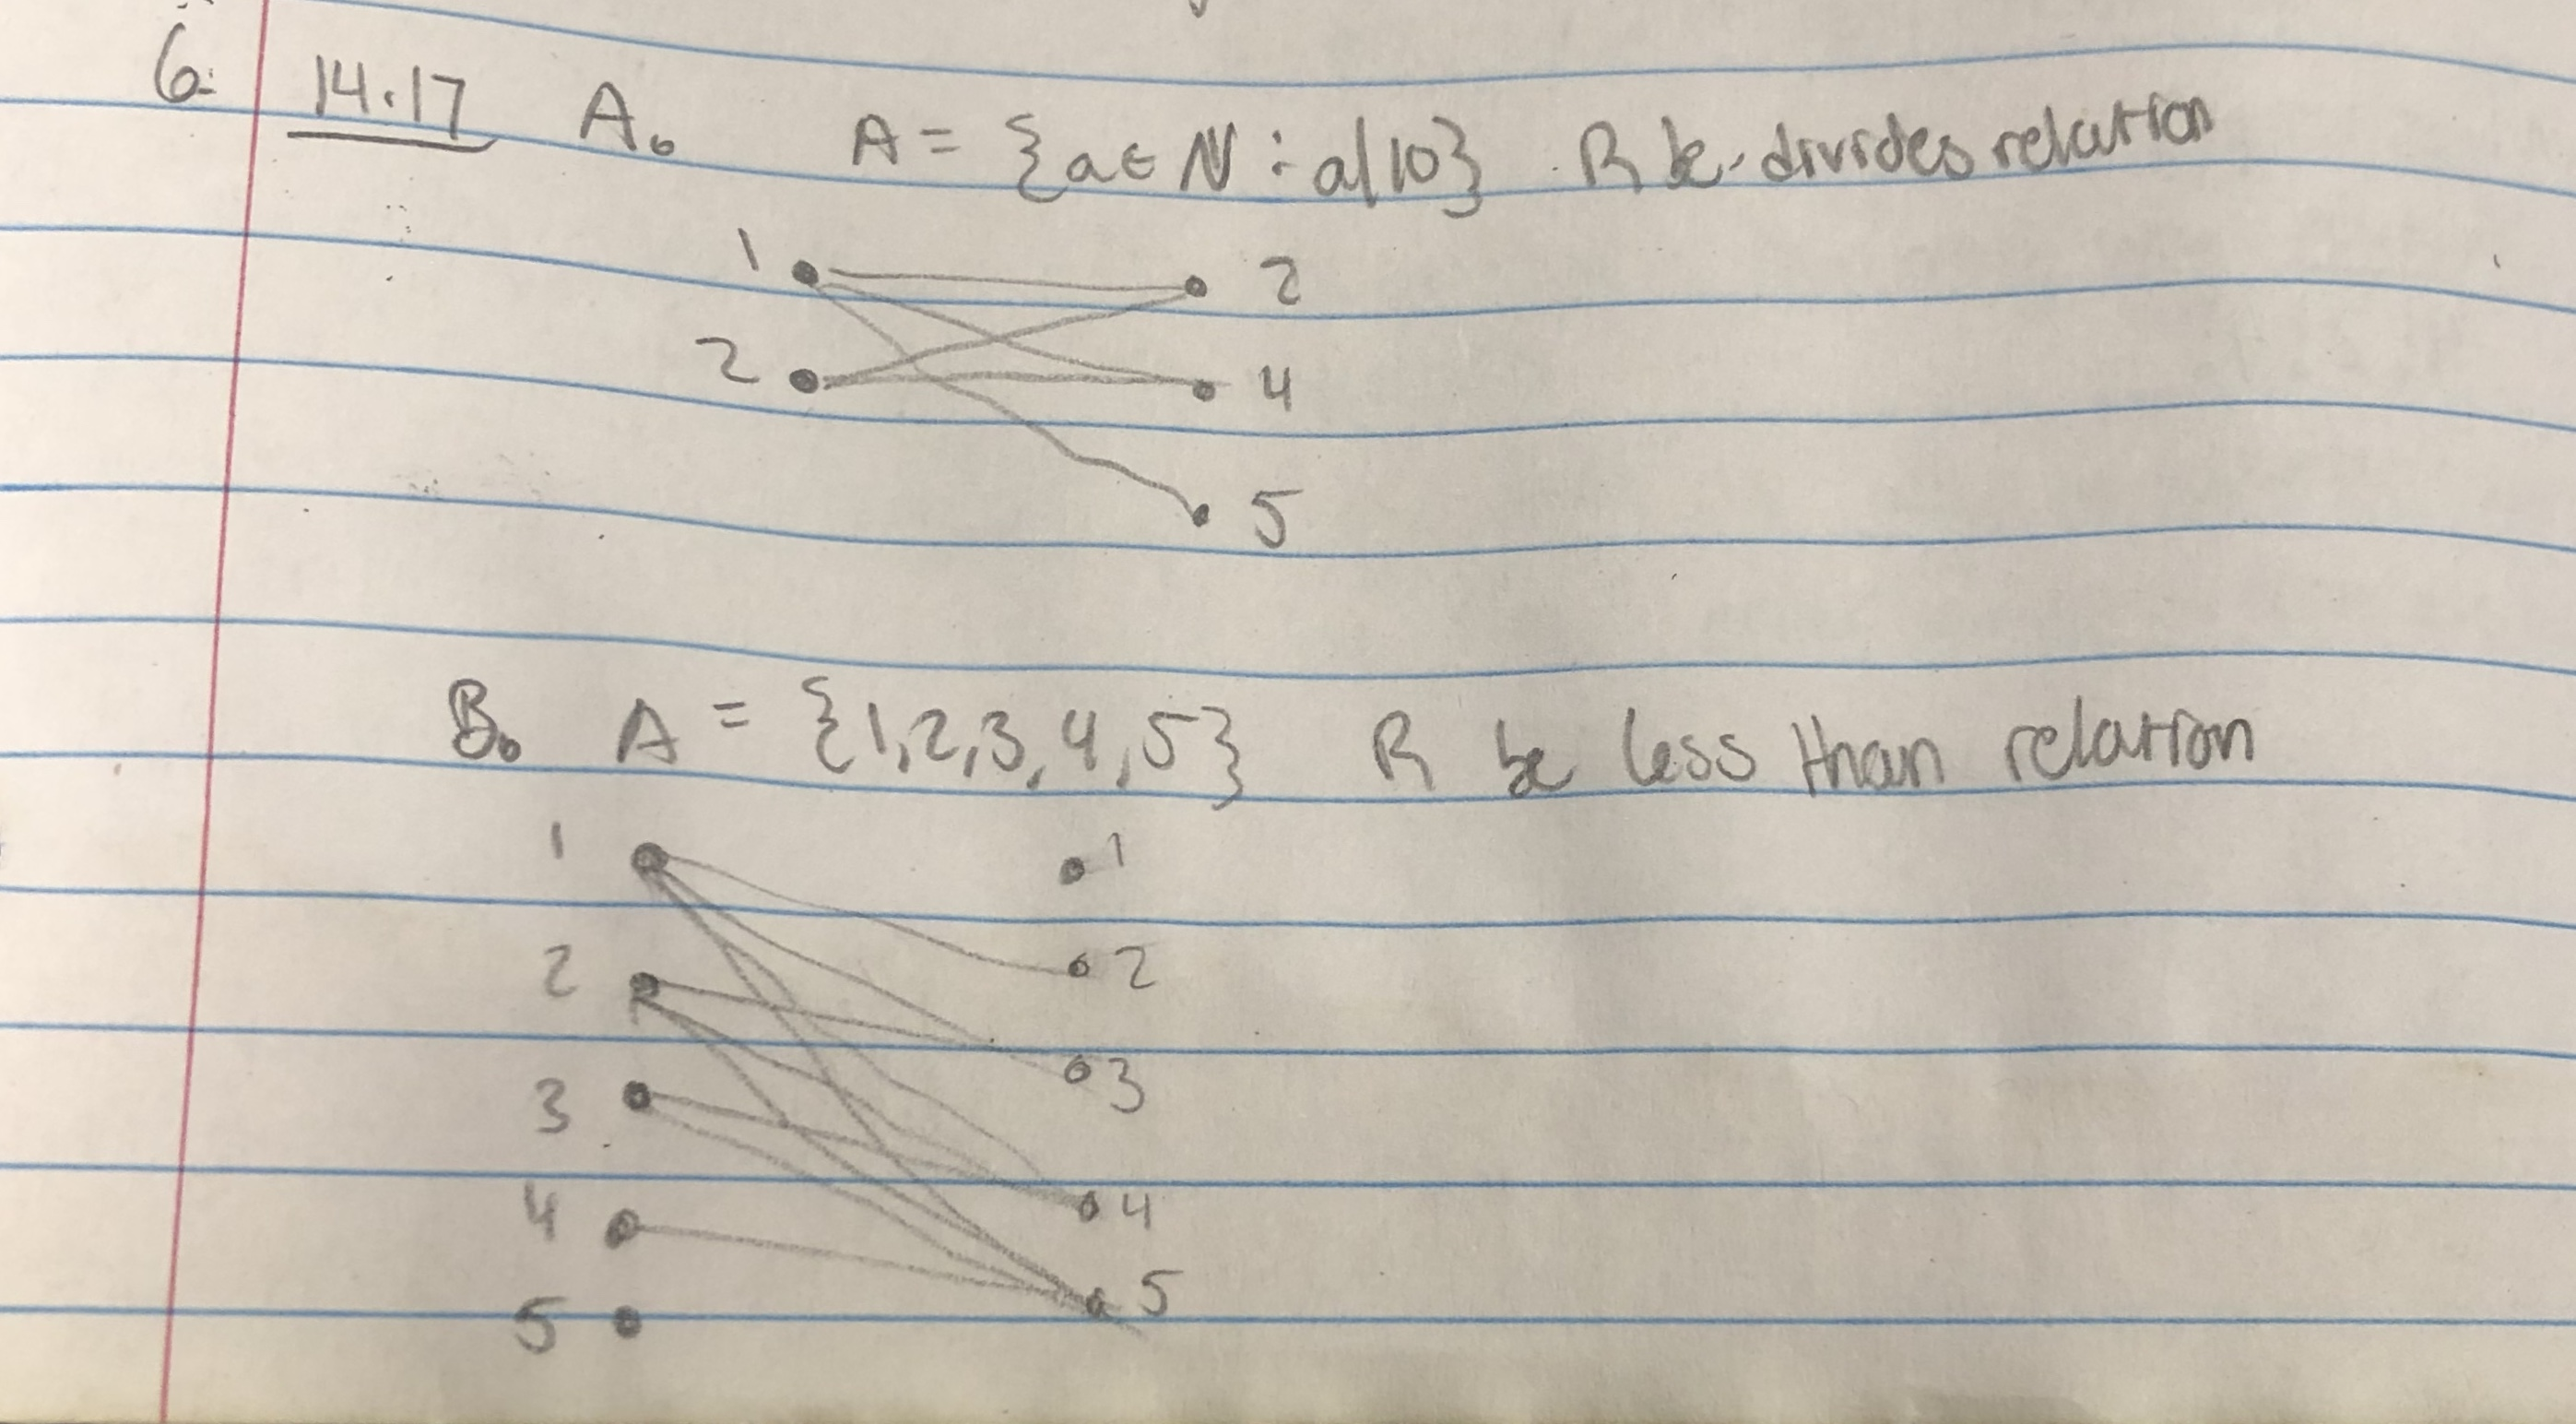
\includegraphics[width = 7in, height = 3in]{HW5_1.jpg} %your jpg file goes between the curly brackets.  To size it, play around with the syntax between the square brackets.  
\] \\ 
\[
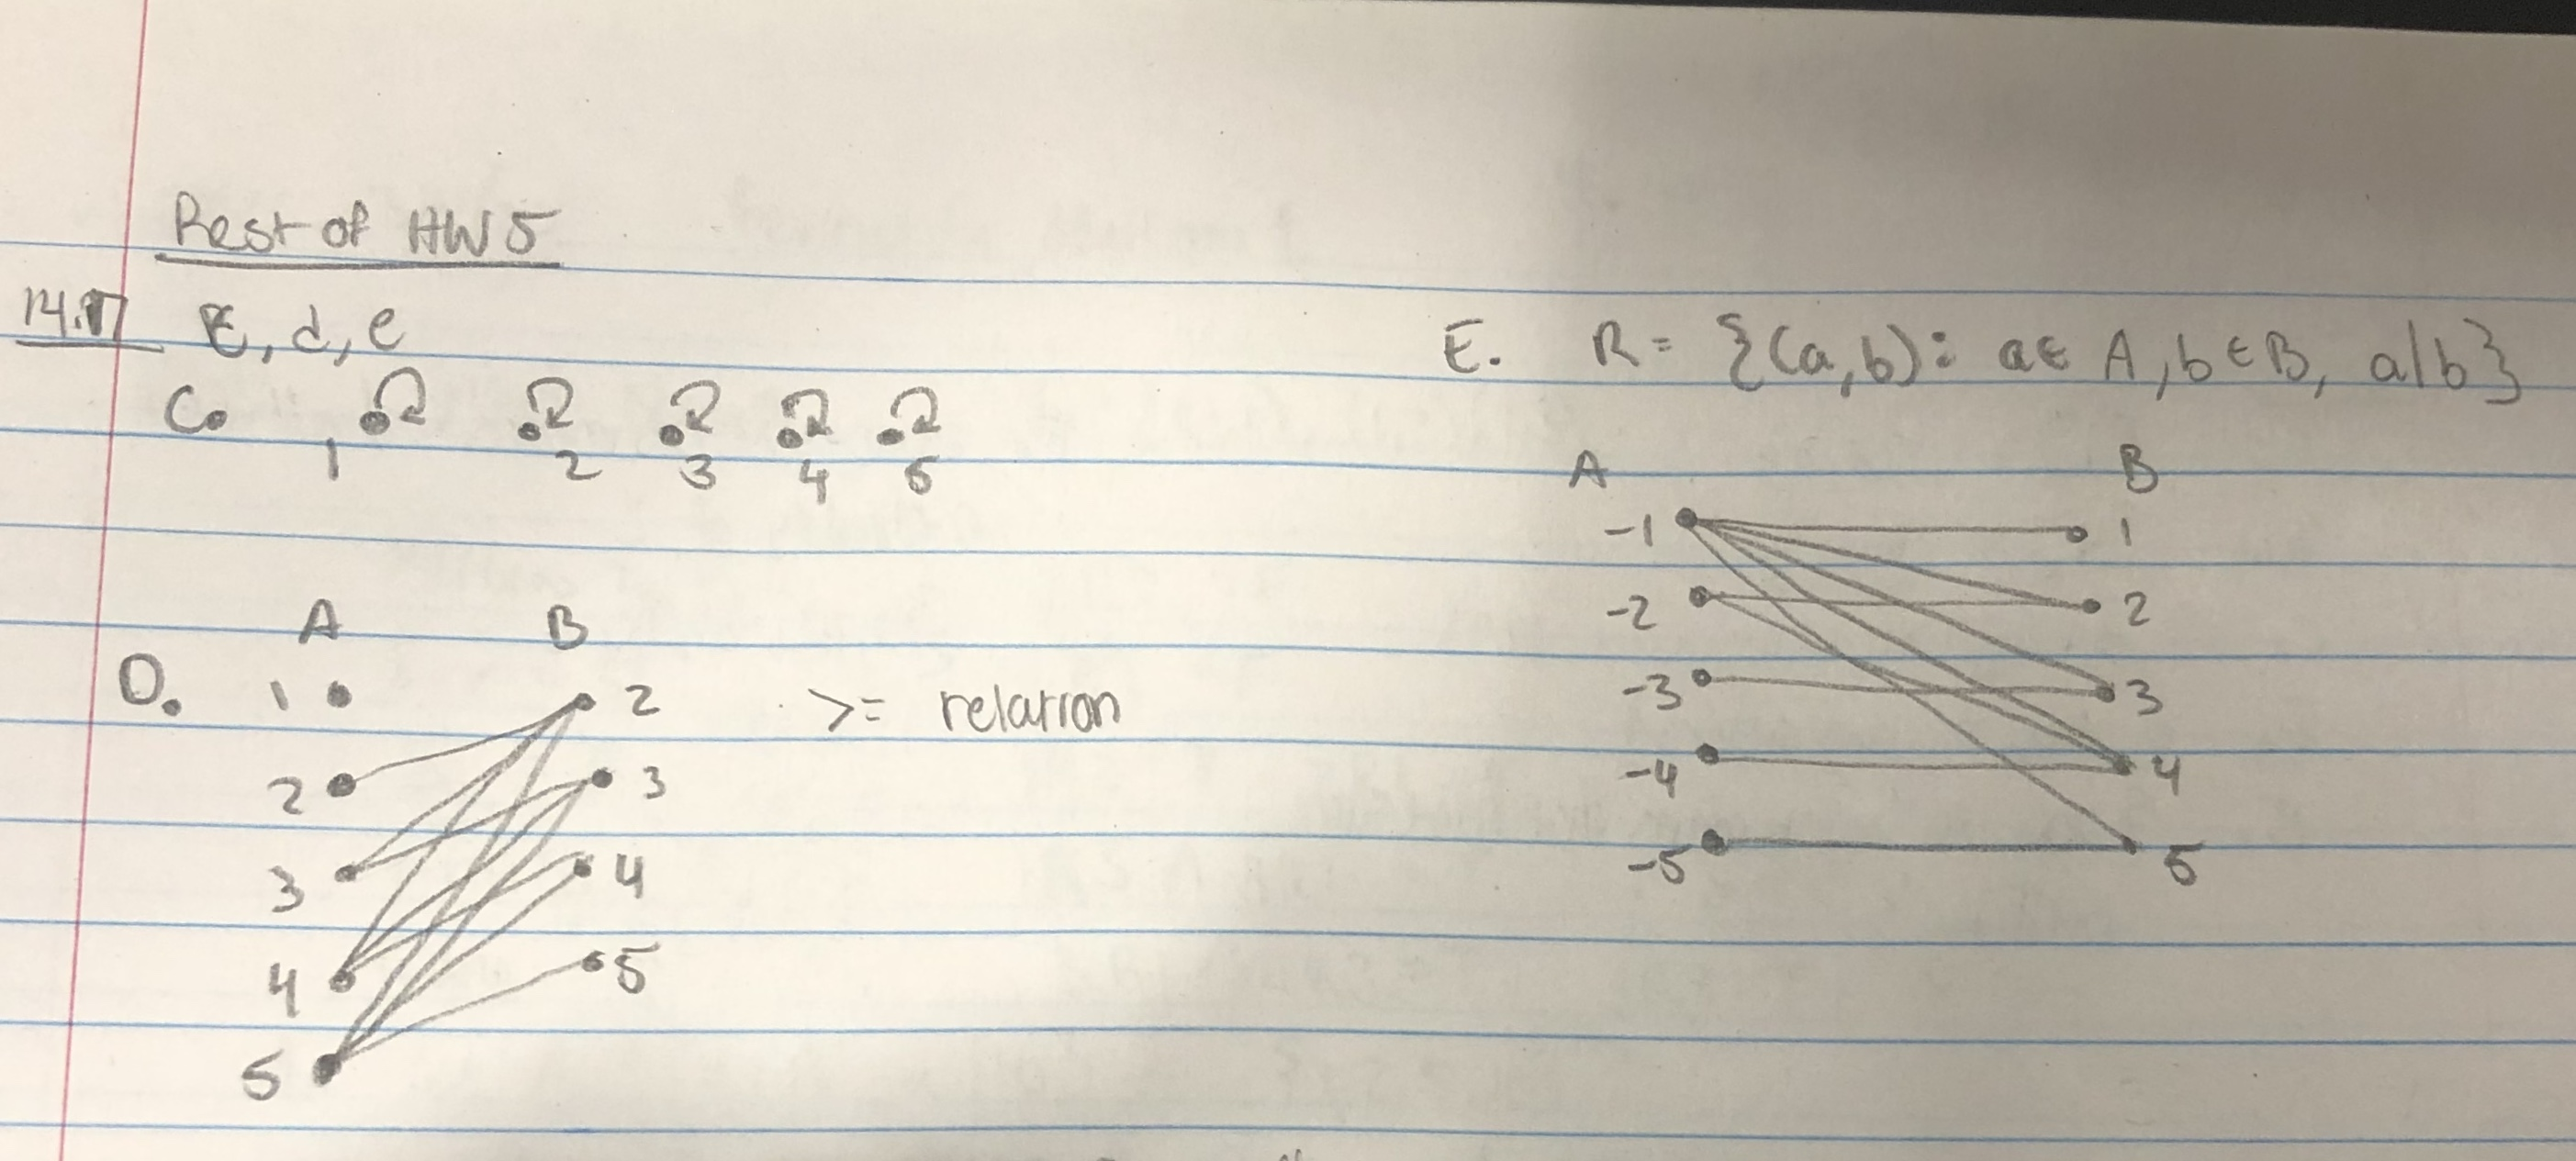
\includegraphics[width = 7in, height = 3in]{HW5_2.jpg} %your jpg file goes between the curly brackets.  To size it, play around with the syntax between the square brackets.  
\]